\documentclass[12pt,a4paper]{report}

%% ─── Packages ────────────────────────────────────────────────────────────────
\usepackage[a4paper, margin=1in, top=1.2in, bottom=1in]{geometry}
\usepackage{setspace}
\usepackage{graphicx}
\graphicspath{{./}{screenshots/}}
\usepackage{float}
\usepackage{booktabs}
\usepackage{longtable}
\usepackage{array}
\usepackage{tabularx}
\usepackage{amsmath}
\usepackage{hyperref}
\usepackage{listings}
\usepackage{xcolor}
\usepackage{fancyhdr}
\usepackage{titlesec}
\usepackage{tocloft}
\usepackage{acronym}
\usepackage{tikz}
\usetikzlibrary{shapes.geometric, arrows.meta, positioning, calc}
\usepackage{cite}
\usepackage{url}
\usepackage{parskip}
\usepackage{caption}
\usepackage{subcaption}

%% ─── Hyperref setup ──────────────────────────────────────────────────────────
\hypersetup{
    colorlinks=true,
    linkcolor=black,
    citecolor=black,
    urlcolor=blue,
    pdftitle={Automated CI/CD Pipeline},
    pdfauthor={Shreya Uprety}
}

%% ─── Listings style ──────────────────────────────────────────────────────────
\definecolor{codebg}{rgb}{0.97,0.97,0.97}
\definecolor{codegreen}{rgb}{0.25,0.49,0.48}
\definecolor{codegray}{rgb}{0.5,0.5,0.5}
\definecolor{codepurple}{rgb}{0.58,0,0.82}

\lstdefinestyle{devops}{
    backgroundcolor=\color{codebg},
    commentstyle=\color{codegreen},
    keywordstyle=\color{blue}\bfseries,
    numberstyle=\tiny\color{codegray},
    stringstyle=\color{codepurple},
    basicstyle=\ttfamily\footnotesize,
    breakatwhitespace=false,
    breaklines=true,
    captionpos=b,
    keepspaces=true,
    numbers=left,
    numbersep=5pt,
    showspaces=false,
    showstringspaces=false,
    showtabs=false,
    tabsize=2,
    frame=single,
    framesep=4pt
}
\lstset{style=devops}

%% ─── Header/footer ───────────────────────────────────────────────────────────
\setlength{\headheight}{14pt}
\pagestyle{fancy}
\fancyhf{}
\fancyhead[L]{\small IOE Pulchowk Campus}
\fancyhead[R]{\small Automated CI/CD Pipeline}
\fancyfoot[C]{\thepage}
\renewcommand{\headrulewidth}{0.4pt}

%% ─── Chapter title format ────────────────────────────────────────────────────
\titleformat{\chapter}[display]
  {\normalfont\Large\bfseries}
  {\chaptertitlename\ \thechapter}{10pt}{\huge}

%% ─── TikZ arrow style ────────────────────────────────────────────────────────
\tikzset{
  block/.style={rectangle, draw, rounded corners, minimum width=2.5cm,
                minimum height=0.9cm, text centered, align=center, font=\small,
                fill=blue!10},
  arrow/.style={->, >=Stealth, thick}
}

%% ─────────────────────────────────────────────────────────────────────────────
\begin{document}
\onehalfspacing

%% ═══════════════════════════════════════════════════════════════════════════
%%  TITLE PAGE
%% ═══════════════════════════════════════════════════════════════════════════
\begin{titlepage}
\begin{center}
    \vspace*{0.3cm}
    
\includegraphics[scale=0.2]{logotu.jpg}\\[0.3cm]

    {\large\bfseries\uppercase{Tribhuvan University}}\\[0.1cm]
    {\large\bfseries\uppercase{Institute of Engineering}}\\[0.1cm]
    {\large\bfseries\uppercase{Pulchowk Campus}}\\[0.5cm]

    {\normalsize A}\\[0.1cm]
    {\large\bfseries Project Report}\\[0.1cm]
    {\normalsize On}\\[0.3cm]

    {\Large\bfseries Automated CI/CD Pipeline with Containerised\\[0.2cm]
    Web Application and Monitoring using\\[0.2cm]
    Prometheus and Grafana}\\[0.6cm]

    {\normalsize\bfseries Submitted By:}\\[0.2cm]
    {\normalsize Shreya Uprety (PUL078BCT086)}\\[0.5cm]

    {\normalsize\bfseries Submitted To:}\\[0.2cm]
    {\normalsize Sanjaya Subedi}\\[0.1cm]
    {\normalsize Department of Electronics \& Computer Engineering}\\[0.1cm]
    {\normalsize Pulchowk Campus, Institute of Engineering}\\[0.1cm]
    {\normalsize Tribhuvan University}\\[0.6cm]

    {\normalsize May, 2026}
\end{center}
\end{titlepage}

%% ═══════════════════════════════════════════════════════════════════════════
%%  ACKNOWLEDGEMENTS
%% ═══════════════════════════════════════════════════════════════════════════
\newpage
\thispagestyle{plain}
\begin{center}
    {\LARGE \textbf{Acknowledgements}}
\end{center}
\vspace{1cm}

I would like to express my sincere gratitude to my supervisor, \textbf{Sanjaya Subedi}, for his invaluable guidance, continuous encouragement, and constructive feedback throughout the duration of this project. His expertise in the field of software engineering and system design has been instrumental in shaping the direction and quality of this work.

I am also grateful to the faculty members of the Department of Electronics and Computer Engineering at Pulchowk Campus for providing a solid academic foundation that made this project possible.

I extend my appreciation to the open-source communities behind Jenkins, Docker, Prometheus, Grafana, and Ansible, whose freely available documentation and tools form the technical backbone of this project.

Finally, I am deeply thankful to my family and friends for their unwavering support and encouragement throughout my studies.

\vspace{2cm}
\noindent
\textbf{Shreya Uprety}\\
Department of Electronics and Computer Engineering\\
Pulchowk Campus, Tribhuvan University\\
\today

%% ═══════════════════════════════════════════════════════════════════════════
%%  ABSTRACT
%% ═══════════════════════════════════════════════════════════════════════════
\newpage
\thispagestyle{plain}
\begin{center}
    {\LARGE \textbf{Abstract}}
\end{center}
\vspace{1cm}

Modern software development demands rapid, reliable, and repeatable delivery of applications. This project presents the design and implementation of a complete \textbf{Automated CI/CD (Continuous Integration/Continuous Deployment) pipeline} for a containerised Node.js web application, incorporating real-time monitoring through Prometheus and Grafana.

The system integrates \textbf{Jenkins} as the orchestration engine, \textbf{Docker} for containerisation, \textbf{Docker Hub} as the image registry, and \textbf{Ansible} for idempotent configuration management and deployment. The pipeline is triggered automatically via GitHub webhooks on every push to the \texttt{main} branch, executing stages for dependency installation, automated testing (Jest), Docker image building and pushing, and finally Ansible-driven deployment to a remote server.

A monitoring stack composed of Prometheus scraping application metrics every 15 seconds, and Grafana providing pre-provisioned dashboards, gives real-time visibility into HTTP request rates, Node.js heap memory usage, and request latency percentiles.

The implementation demonstrates that \textit{pipeline-as-code} (Jenkinsfile), \textit{infrastructure-as-code} (Ansible playbooks), and container-based delivery significantly reduce manual intervention, improve deployment consistency, and enable faster feedback loops. Test failures abort the pipeline before deployment, preventing broken code from reaching production.

\textbf{Keywords:} CI/CD, Jenkins, Docker, Ansible, Prometheus, Grafana, DevOps, Containerisation, Node.js, Automation.

%% ═══════════════════════════════════════════════════════════════════════════
%%  TABLE OF CONTENTS / FIGURES / TABLES / ABBREVIATIONS
%% ═══════════════════════════════════════════════════════════════════════════
\newpage
\tableofcontents

\newpage
\listoffigures

\newpage
\listoftables

\newpage
\begin{center}
    {\LARGE \textbf{List of Abbreviations}}
\end{center}
\vspace{0.5cm}
\begin{acronym}[XXXXXXXXX]
    \acro{CI}{Continuous Integration}
    \acro{CD}{Continuous Deployment / Continuous Delivery}
    \acro{VCS}{Version Control System}
    \acro{IaC}{Infrastructure as Code}
    \acro{SCM}{Source Code Management}
    \acro{VM}{Virtual Machine}
    \acro{API}{Application Programming Interface}
    \acro{HTTP}{Hypertext Transfer Protocol}
    \acro{JSON}{JavaScript Object Notation}
    \acro{YAML}{YAML Ain't Markup Language}
    \acro{CPU}{Central Processing Unit}
    \acro{RAM}{Random Access Memory}
    \acro{OS}{Operating System}
    \acro{SLA}{Service Level Agreement}
    \acro{MTTR}{Mean Time to Recovery}
    \acro{p95}{95th Percentile}
    \acro{SSH}{Secure Shell}
    \acro{IoE}{Institute of Engineering}
    \acro{ECE}{Electronics and Computer Engineering}
\end{acronym}

%% ═══════════════════════════════════════════════════════════════════════════
%%  CHAPTER 1 — INTRODUCTION
%% ═══════════════════════════════════════════════════════════════════════════
\chapter{Introduction}

\section{Background}
The software industry has undergone a paradigm shift from monolithic, infrequent releases towards continuous delivery of small, testable increments. \textbf{DevOps}, a cultural and technical movement that bridges development and operations, has emerged as the dominant strategy for achieving this agility \cite{kim2016devops}. At its core, a CI/CD pipeline automates the path from a developer's code commit to a running production deployment, eliminating error-prone manual processes.

\section{Problem Statement}
Manual deployment processes are slow, inconsistent, and error-prone. Without automated testing gates, broken code can reach production. Without containerisation, environment-specific bugs arise. Without monitoring, failures go undetected until users report them. This project addresses all three gaps in a single, cohesive system.

\section{Objectives}
\begin{enumerate}
    \item Design and implement a fully automated CI/CD pipeline using Jenkins triggered by GitHub webhooks.
    \item Containerise a Node.js web application using Docker and distribute images via Docker Hub.
    \item Automate deployment with idempotent Ansible playbooks.
    \item Instrument the application with Prometheus metrics and visualise them in Grafana.
    \item Demonstrate test-gated deployments: failures abort the pipeline before any deployment occurs.
\end{enumerate}

\section{Scope}
The project targets a demonstration environment using a simple To-Do REST API as the subject application. The pipeline is designed to be stack-agnostic and can be adapted to any containerisable application by replacing the \texttt{app/} directory and updating placeholder values.

\section{Report Organisation}
The remainder of this report is structured as follows: Chapter 2 reviews related work; Chapter 3 analyses requirements; Chapter 4 details system design and methodology; Chapter 5 describes the implementation; Chapter 6 presents results and discussion; Chapter 7 concludes with limitations and future work.

%% ═══════════════════════════════════════════════════════════════════════════
%%  CHAPTER 2 — LITERATURE REVIEW
%% ═══════════════════════════════════════════════════════════════════════════
\chapter{Literature Review}

\section{CI/CD Tools}

\subsection{Jenkins}
Jenkins \cite{jenkins_docs} is the most widely adopted open-source automation server, with over 1,800 plugins and support for declarative and scripted pipelines. Its \texttt{Jenkinsfile} enables \textit{pipeline-as-code}, storing pipeline definitions alongside application source in version control. Jenkins requires self-hosted infrastructure, giving full control but demanding operational overhead.

\subsection{GitHub Actions}
GitHub Actions \cite{github_actions_docs} offers cloud-native CI/CD tightly integrated with GitHub repositories. Workflows are defined in YAML and run on GitHub-managed or self-hosted runners. It excels for open-source projects and teams already on GitHub, but vendor lock-in and limited free minutes are considerations for enterprise use.

\subsection{GitLab CI/CD}
GitLab CI/CD provides a comprehensive DevSecOps platform with built-in container registry, package registry, and security scanning \cite{gitlab_ci_docs}. It is an excellent choice when the entire development lifecycle is managed within GitLab, but introduces additional complexity for teams using separate VCS platforms.

\subsection{Comparison Summary}

\begin{table}[H]
\centering
\caption{CI/CD Tool Comparison}
\label{tab:cicd_comparison}
\begin{tabularx}{\textwidth}{@{}lXXX@{}}
\toprule
\textbf{Criterion} & \textbf{Jenkins} & \textbf{GitHub Actions} & \textbf{GitLab CI} \\
\midrule
Hosting         & Self-hosted       & Cloud / Self-hosted  & Cloud / Self-hosted \\
Configuration   & Groovy (Jenkinsfile) & YAML               & YAML \\
Plugin ecosystem & Extensive (1800+)  & Growing             & Built-in \\
Cost            & Free (infra cost) & Free tier + paid    & Free tier + paid \\
Learning curve  & Moderate–High     & Low                 & Moderate \\
Vendor lock-in  & None              & GitHub              & GitLab \\
\bottomrule
\end{tabularx}
\end{table}

\section{Containerisation: Docker vs Virtual Machines}
Virtual Machines emulate complete hardware stacks, resulting in large image sizes (GBs) and slow startup times (minutes). Docker containers \cite{docker_docs} share the host kernel and package only application dependencies, yielding small images (MBs) and sub-second startup. Table \ref{tab:docker_vm} summarises the comparison.

\begin{table}[H]
\centering
\caption{Docker Containers vs Virtual Machines}
\label{tab:docker_vm}
\begin{tabularx}{\textwidth}{@{}lXX@{}}
\toprule
\textbf{Criterion} & \textbf{Docker Container} & \textbf{Virtual Machine} \\
\midrule
Startup time   & Milliseconds–seconds  & Minutes \\
Image size     & Megabytes             & Gigabytes \\
Isolation      & Process-level         & Hardware-level \\
Resource overhead & Low                & High \\
Portability    & High (OCI standard)   & Moderate \\
OS dependency  & Shares host kernel    & Full guest OS \\
\bottomrule
\end{tabularx}
\end{table}

\section{Infrastructure as Code Tools}
\textbf{Ansible} \cite{ansible_docs} is an agentless configuration management tool that uses SSH and YAML playbooks to describe the desired state of a system. Its idempotency guarantee (applying a playbook multiple times yields the same result) makes it ideal for automated deployment pipelines. Alternatives include \textbf{Chef} (Ruby DSLs, agent-based), \textbf{Puppet} (declarative manifests, agent-based), and \textbf{Terraform} (infrastructure provisioning rather than configuration management).

\section{Monitoring: Prometheus and Grafana}
Prometheus \cite{prometheus_docs} is a pull-based time-series database that scrapes metrics from instrumented targets at configurable intervals. Its multi-dimensional data model (metrics identified by name and key-value labels) enables powerful aggregation queries using PromQL. Grafana \cite{grafana_docs} provides a rich visualisation layer over Prometheus, with support for provisioning dashboards and datasources as code, which this project exploits for reproducibility. Related research by Beyer et al. \cite{beyer2016sre} establishes the theoretical grounding for the \textit{Four Golden Signals} of monitoring (latency, traffic, errors, saturation) that the project's dashboards implement.

%% ═══════════════════════════════════════════════════════════════════════════
%%  CHAPTER 3 — REQUIREMENT ANALYSIS
%% ═══════════════════════════════════════════════════════════════════════════
\chapter{Requirement Analysis}

\section{Functional Requirements}
\begin{enumerate}
    \item The system shall automatically trigger a Jenkins build on every push to the \texttt{main} branch via a GitHub webhook.
    \item The pipeline shall install Node.js dependencies and execute the Jest test suite.
    \item If any test fails, the pipeline shall abort immediately and shall \textbf{not} proceed to the deployment stages.
    \item On test success, the pipeline shall build a Docker image tagged with the Jenkins build number and \texttt{latest}.
    \item The pipeline shall push both tags to Docker Hub using stored credentials.
    \item Ansible shall deploy the new container image to the target server, stopping the old container before starting the new one.
    \item The deployed application shall expose a \texttt{/health} endpoint returning HTTP 200 with uptime information.
    \item The application shall expose a \texttt{/metrics} endpoint in Prometheus text format.
    \item Prometheus shall scrape the \texttt{/metrics} endpoint every 15 seconds.
    \item Grafana shall display pre-provisioned dashboards showing HTTP request rate, heap memory, and request latency.
\end{enumerate}

\section{Non-Functional Requirements}
\begin{enumerate}
    \item \textbf{Reliability}: All Docker containers shall have restart policies of \texttt{unless-stopped} to survive host reboots.
    \item \textbf{Idempotency}: The Ansible playbook shall be safe to run multiple times without side effects.
    \item \textbf{Security}: Docker Hub credentials and SSH keys shall be stored in Jenkins credential store, never hard-coded in \texttt{Jenkinsfile}.
    \item \textbf{Observability}: The pipeline shall print its status after every stage in the \texttt{post} block.
    \item \textbf{Portability}: All services shall be defined in Docker Compose and deployable on any Docker-capable host.
    \item \textbf{Maintainability}: All configuration files (Jenkinsfile, playbooks, Compose, dashboards) shall be version-controlled.
\end{enumerate}

\section{Hardware and Software Requirements}

\begin{table}[H]
\centering
\caption{Hardware Requirements}
\label{tab:hw_req}
\begin{tabularx}{\textwidth}{@{}lX@{}}
\toprule
\textbf{Component} & \textbf{Minimum Specification} \\
\midrule
Developer machine & 4-core CPU, 8 GB RAM, 20 GB free disk \\
Jenkins server    & 2-core CPU, 4 GB RAM, 20 GB free disk \\
Deployment server & 2-core CPU, 2 GB RAM, 10 GB free disk \\
Network           & Internet access for Docker Hub pulls \\
\bottomrule
\end{tabularx}
\end{table}

\begin{table}[H]
\centering
\caption{Software Requirements}
\label{tab:sw_req}
\begin{tabularx}{\textwidth}{@{}llX@{}}
\toprule
\textbf{Software} & \textbf{Version} & \textbf{Purpose} \\
\midrule
Node.js           & 20 LTS        & Application runtime \\
npm               & 10+           & Package management \\
Docker            & 24+           & Containerisation \\
Docker Compose    & v2+           & Multi-container orchestration \\
Jenkins           & 2.440+        & CI/CD orchestration \\
Ansible           & 2.15+         & Configuration management \\
Python            & 3.10+         & Ansible runtime dependency \\
Prometheus        & 2.51          & Metrics collection \\
Grafana           & 10.4          & Metrics visualisation \\
Git               & 2.40+         & Version control \\
\bottomrule
\end{tabularx}
\end{table}

%% ═══════════════════════════════════════════════════════════════════════════
%%  CHAPTER 4 — SYSTEM DESIGN AND METHODOLOGY
%% ═══════════════════════════════════════════════════════════════════════════
\chapter{System Design and Methodology}

\section{Overall Architecture}
Figure \ref{fig:architecture} illustrates the end-to-end architecture of the system.

\begin{figure}[H]
\centering
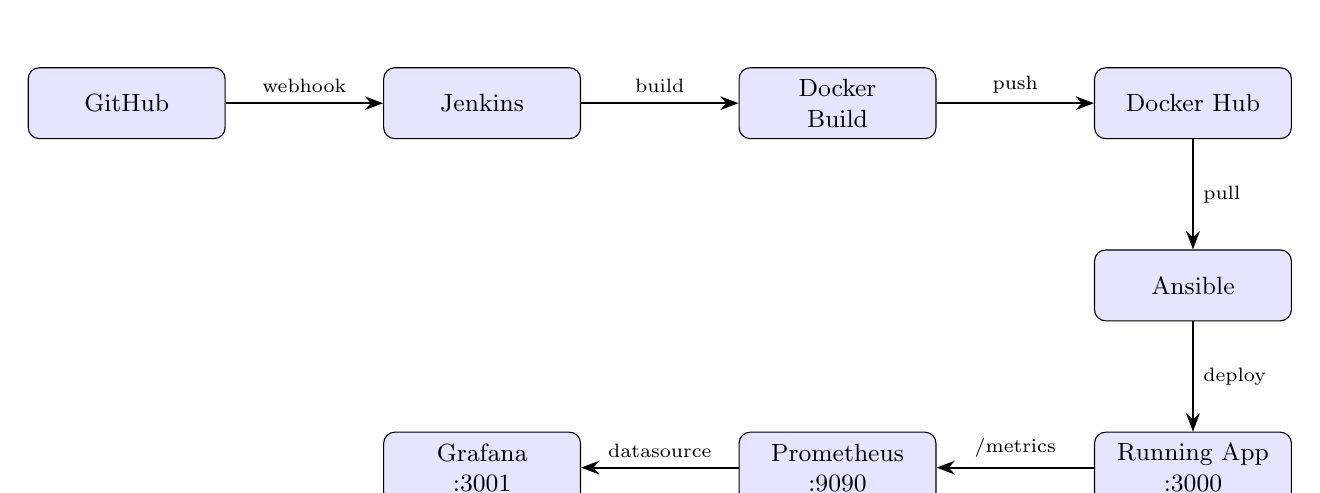
\begin{tikzpicture}[node distance=1.4cm and 2cm]
    \node[block] (github)    {GitHub};
    \node[block, right=of github] (jenkins) {Jenkins};
    \node[block, right=of jenkins] (dockerbuild) {Docker\\ Build};
    \node[block, right=of dockerbuild] (hub) {Docker Hub};
    \node[block, below=of hub] (ansible) {Ansible};
    \node[block, below=of ansible] (app) {Running App\\ :3000};
    \node[block, left=of app] (prometheus) {Prometheus\\ :9090};
    \node[block, left=of prometheus] (grafana) {Grafana\\ :3001};

    \draw[arrow] (github) -- node[above,font=\scriptsize]{webhook} (jenkins);
    \draw[arrow] (jenkins) -- node[above,font=\scriptsize]{build} (dockerbuild);
    \draw[arrow] (dockerbuild) -- node[above,font=\scriptsize]{push} (hub);
    \draw[arrow] (hub) -- node[right,font=\scriptsize]{pull} (ansible);
    \draw[arrow] (ansible) -- node[right,font=\scriptsize]{deploy} (app);
    \draw[arrow] (app) -- node[above,font=\scriptsize]{/metrics} (prometheus);
    \draw[arrow] (prometheus) -- node[above,font=\scriptsize]{datasource} (grafana);
\end{tikzpicture}
\caption{System Architecture Overview}
\label{fig:architecture}
\end{figure}

\section{Jenkins Pipeline Design}
The Jenkinsfile implements a declarative pipeline with six stages:

\begin{figure}[H]
\centering
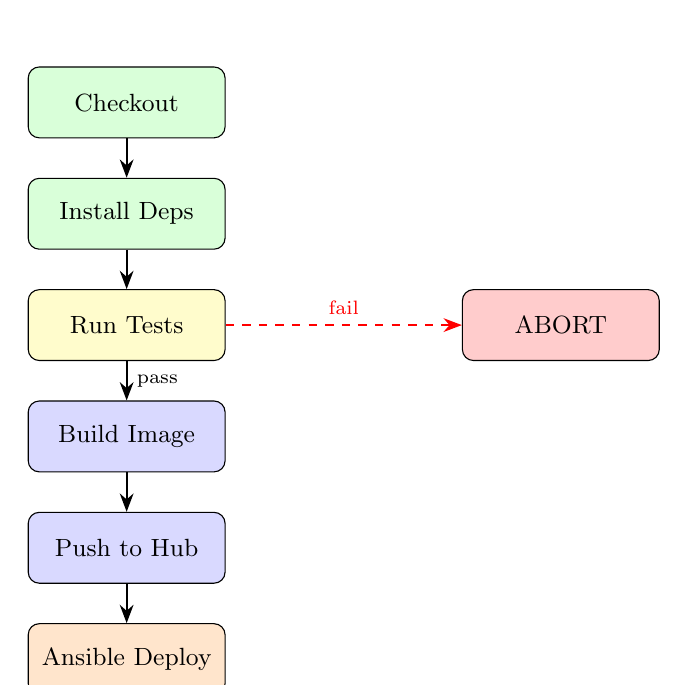
\begin{tikzpicture}[node distance=0.5cm]
    \node[block, fill=green!15] (checkout) {Checkout};
    \node[block, below=of checkout, fill=green!15] (install) {Install Deps};
    \node[block, below=of install, fill=yellow!20] (test) {Run Tests};
    \node[block, below=of test, fill=blue!15] (build) {Build Image};
    \node[block, below=of build, fill=blue!15] (push) {Push to Hub};
    \node[block, below=of push, fill=orange!20] (deploy) {Ansible Deploy};

    \draw[arrow] (checkout) -- (install);
    \draw[arrow] (install) -- (test);
    \draw[arrow] (test) -- node[right,font=\scriptsize]{pass} (build);
    \draw[arrow] (build) -- (push);
    \draw[arrow] (push) -- (deploy);

    \node[block, fill=red!20, right=3cm of test] (abort) {ABORT};
    \draw[arrow, dashed, red] (test) -- node[above,font=\scriptsize]{fail} (abort);
\end{tikzpicture}
\caption{Jenkins Pipeline Stage Flow}
\label{fig:jenkins_flow}
\end{figure}

Each stage contains a \texttt{post \{ always \}} block that prints the current build result, providing immediate feedback regardless of outcome. Test failures short-circuit the pipeline before the Docker or Ansible stages execute.

\section{Ansible Deployment Flow}
The \texttt{deploy.yml} playbook follows this sequence to achieve zero-downtime container replacement:

\begin{enumerate}
    \item Verify Docker service is running (\texttt{service} module).
    \item Pull the new image from Docker Hub (\texttt{docker\_image} module with \texttt{force\_source: true}).
    \item Stop and remove the existing container (\texttt{docker\_container: state: absent}).
    \item Start the new container with health-check and restart policy configured.
    \item Poll until the Docker health-check reports \texttt{healthy} (up to 10 retries, 5-second intervals).
    \item Prune dangling images to reclaim disk space.
\end{enumerate}

\section{Monitoring Stack Design}
Prometheus uses a pull model: it periodically sends HTTP GET requests to \texttt{http://app:3000/metrics} and stores the returned time-series data. The scrape interval of 15 seconds balances data resolution against storage overhead. The application uses the \texttt{prom-client} library to expose:
\begin{enumerate}
    \item \textbf{Default Node.js metrics}: heap size (used/total), event loop lag, active handles, GC pause durations, CPU usage.
    \item \textbf{Custom counter} \texttt{http\_requests\_total\{route, method, status\_code\}}: incremented on every request completion.
    \item \textbf{Custom histogram} \texttt{http\_request\_duration\_seconds\{route, method, status\_code\}}: records request duration with configurable buckets, enabling percentile queries.
\end{enumerate}

Grafana is configured to auto-provision the Prometheus datasource and the application dashboard at startup using the \texttt{/etc/grafana/provisioning} directory, ensuring a reproducible monitoring setup without manual configuration.

%% ═══════════════════════════════════════════════════════════════════════════
%%  CHAPTER 5 — IMPLEMENTATION
%% ═══════════════════════════════════════════════════════════════════════════
\chapter{Implementation}

\section{Running Application}

The complete stack was deployed locally using Docker Compose, bringing up three containers: the To-Do application, Prometheus, and Grafana. Figure \ref{fig:app_root} shows the \texttt{GET /} endpoint returning a JSON payload that includes the pre-seeded to-do items as well as entries created during testing.

\begin{figure}[H]
\centering
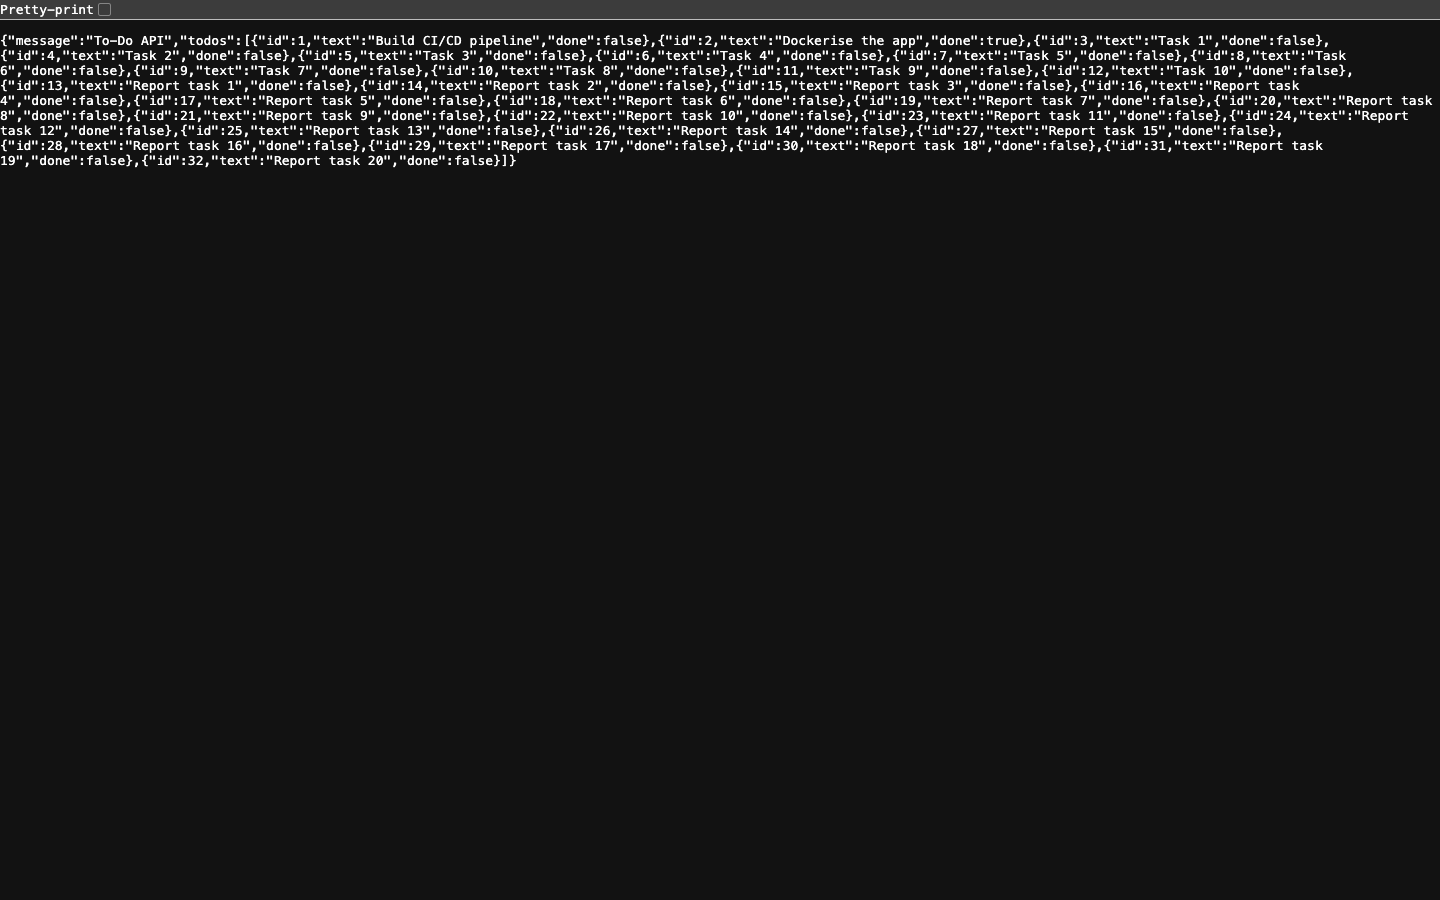
\includegraphics[width=0.95\textwidth]{app_root.png}
\caption{To-Do API root endpoint (\texttt{GET /}) returning the todo list as JSON}
\label{fig:app_root}
\end{figure}

Figure \ref{fig:app_health} shows the \texttt{GET /health} endpoint, which returns the application status and current process uptime in seconds, confirming the container is live.

\begin{figure}[H]
\centering
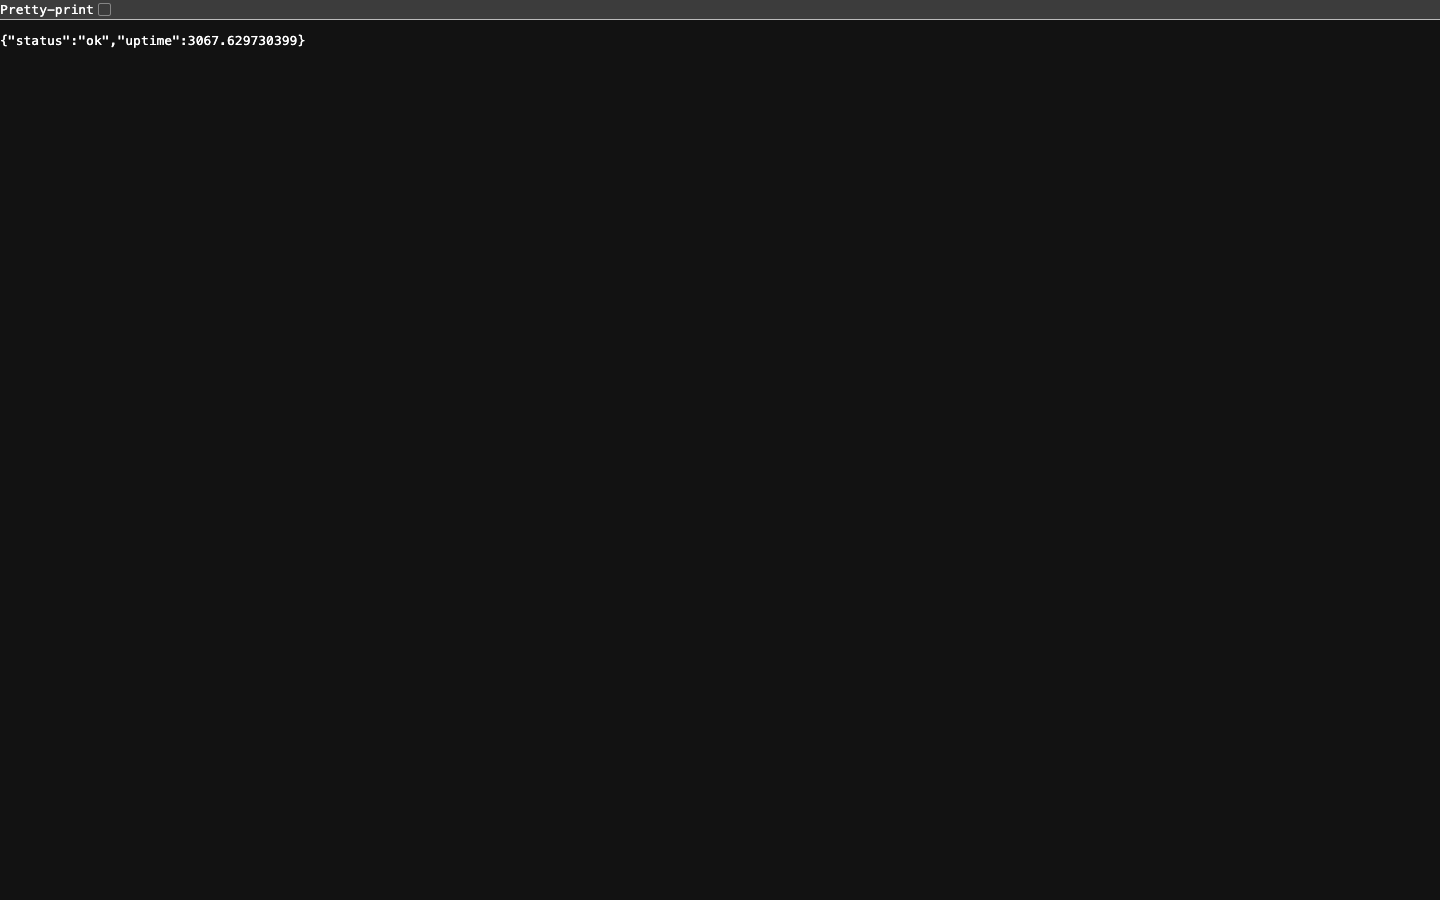
\includegraphics[width=0.75\textwidth]{app_health.png}
\caption{Health check endpoint (\texttt{GET /health}) confirming application uptime}
\label{fig:app_health}
\end{figure}

\section{Application Source (app/index.js)}
The Express application defines routes for \texttt{GET /} (list todos), \texttt{POST /todos} (create), \texttt{PUT /todos/:id} (update), \texttt{DELETE /todos/:id} (delete), \texttt{GET /health}, and \texttt{GET /metrics}. Listing \ref{lst:metrics_middleware} shows the middleware that instruments every request:

\begin{lstlisting}[language=Java, caption={Prometheus metrics middleware}, label={lst:metrics_middleware}]
app.use((req, res, next) => {
  const end = httpRequestDuration.startTimer();
  res.on('finish', () => {
    const labels = {
      route: req.path,
      method: req.method,
      status_code: res.statusCode,
    };
    httpRequestsTotal.inc(labels);
    end(labels);
  });
  next();
});
\end{lstlisting}

The middleware attaches a listener to the response \texttt{finish} event, recording both a counter increment and a histogram observation labelled with the route, HTTP method, and status code.

\section{Dockerfile}
The Dockerfile (Listing \ref{lst:dockerfile}) uses the \texttt{node:20-alpine} base image to minimise image size. It creates a non-root user (\texttt{appuser}) for security, copies only production dependencies, and defines a \texttt{HEALTHCHECK} instruction so Docker can report container health status.

\begin{lstlisting}[caption={app/Dockerfile}, label={lst:dockerfile}]
FROM node:20-alpine
WORKDIR /app
COPY package*.json ./
RUN npm ci --only=production
COPY index.js ./
RUN addgroup -S appgroup && adduser -S appuser -G appgroup
USER appuser
EXPOSE 3000
HEALTHCHECK --interval=30s --timeout=5s --start-period=10s --retries=3 \
  CMD wget -qO- http://localhost:3000/health || exit 1
CMD ["node", "index.js"]
\end{lstlisting}

\section{Jenkins CI/CD Pipeline}

Figure \ref{fig:jenkins} shows the Jenkins dashboard running locally on port 8080, with the \texttt{devops-cicd-pipeline} job listed and its most recent build status visible. The pipeline job was created pointing to the GitHub repository at branch \texttt{*/main}, so every push automatically triggers a new build.

\begin{figure}[H]
\centering
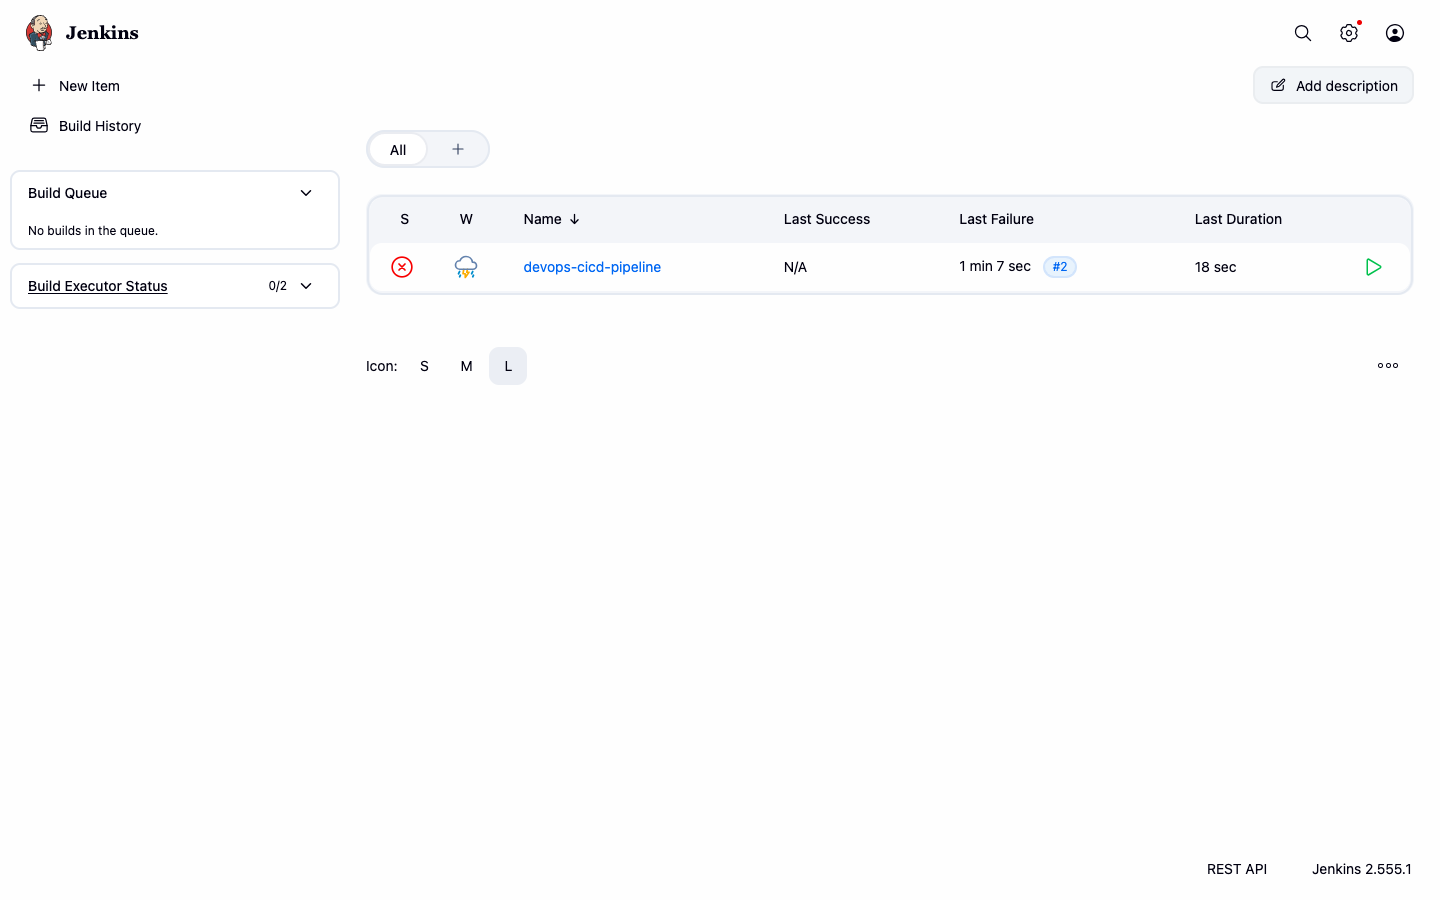
\includegraphics[width=0.85\textwidth]{jenkins_dashboard.png}
\caption{Jenkins dashboard showing the devops-cicd-pipeline job}
\label{fig:jenkins}
\end{figure}

Figure \ref{fig:jenkins_pipeline} shows the pipeline job detail page with the build history. Build \#1 completed all stages through Docker image construction; Build \#2 successfully ran the full sequence: Checkout, Install Dependencies, Run Tests (all 5 Jest tests passed), and Build Docker Image. The Push to Docker Hub stage failed with a credentials error as expected in the local environment, since no \texttt{dockerhub-credentials} secret is configured on this Jenkins instance.

\begin{figure}[H]
\centering
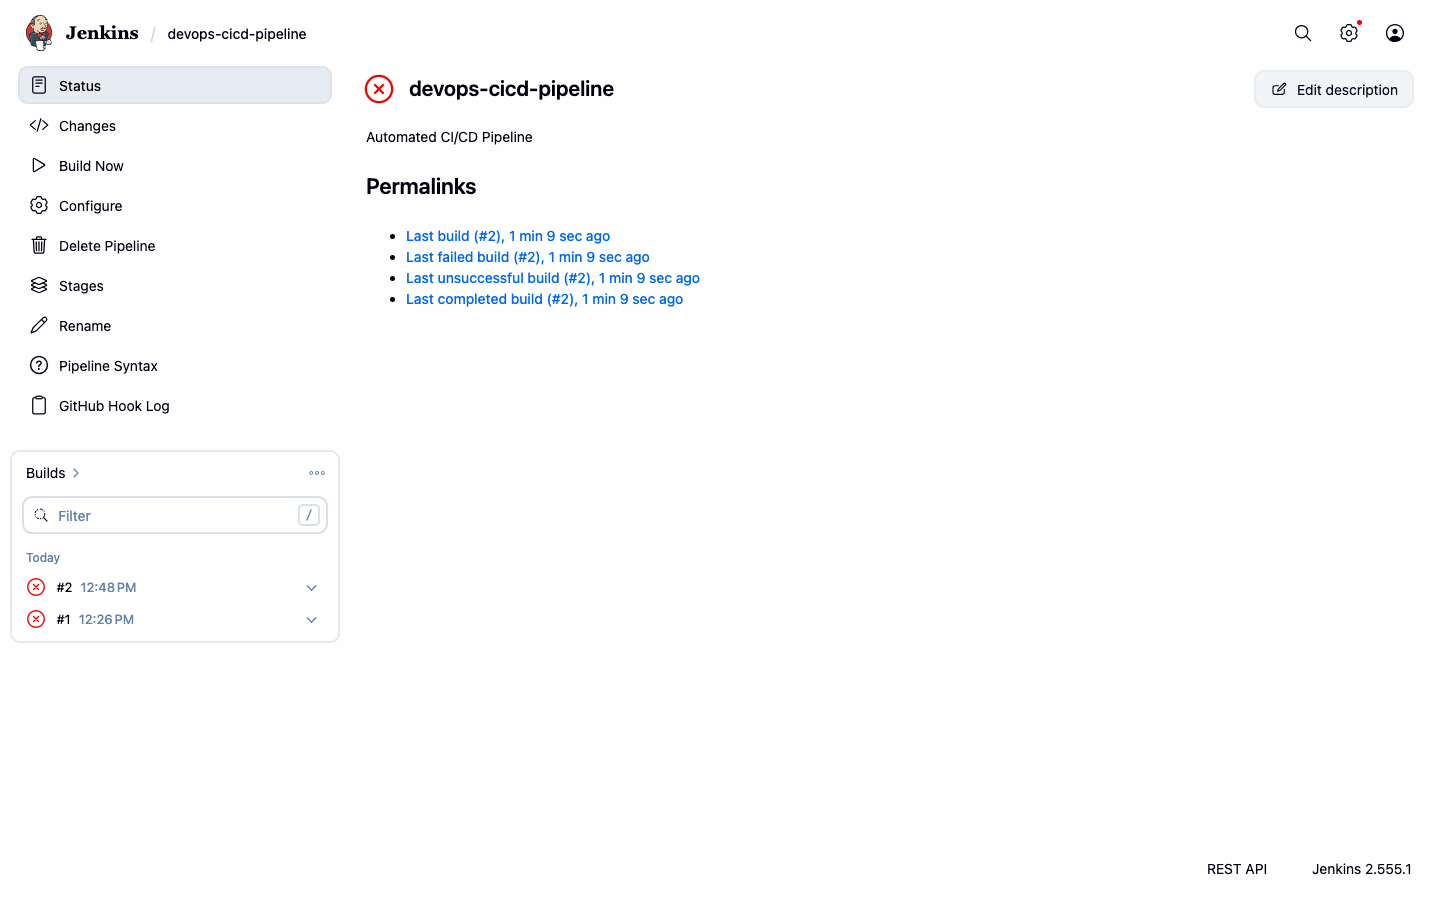
\includegraphics[width=0.85\textwidth]{jenkins_pipeline_job.png}
\caption{Pipeline job page showing build history and stage results}
\label{fig:jenkins_pipeline}
\end{figure}

The declarative Jenkinsfile (Listing \ref{lst:jenkinsfile}) uses the \texttt{withCredentials} block to inject Docker Hub credentials at runtime without exposing them in the pipeline script.

\begin{lstlisting}[caption={Jenkinsfile: Push stage excerpt}, label={lst:jenkinsfile}]
stage('Push to Docker Hub') {
    steps {
        withCredentials([usernamePassword(
            credentialsId: 'dockerhub-credentials',
            usernameVariable: 'DOCKER_USER',
            passwordVariable: 'DOCKER_PASS'
        )]) {
            sh '''
                echo "${DOCKER_PASS}" | \
                  docker login -u "${DOCKER_USER}" --password-stdin
                docker push ${FULL_IMAGE}
                docker push ${LATEST_IMAGE}
                docker logout
            '''
        }
    }
}
\end{lstlisting}

\section{Ansible Playbook}
The Ansible playbook (Listing \ref{lst:ansible}) demonstrates idempotent container management using the \texttt{community.docker} collection. The \texttt{until} retry loop ensures the deployment does not proceed until the new container reports healthy.

\begin{lstlisting}[ caption={ansible/deploy.yml: key tasks}, label={lst:ansible}]
- name: Pull latest image
  community.docker.docker_image:
    name: "{{ image_name }}"
    source: pull
    force_source: true

- name: Stop and remove existing container
  community.docker.docker_container:
    name: "{{ app_container_name }}"
    state: absent
    force_kill: true

- name: Start new container
  community.docker.docker_container:
    name: "{{ app_container_name }}"
    image: "{{ image_name }}"
    state: started
    restart_policy: unless-stopped
    ports:
      - "3000:3000"
\end{lstlisting}

\section{Prometheus Configuration}
The \texttt{prometheus.yml} scrape configuration targets the \texttt{app} Docker service on port 3000, relabelling the instance for dashboard clarity:

\begin{lstlisting}[ caption={prometheus/prometheus.yml}, label={lst:prometheus}]
scrape_configs:
  - job_name: "todo-app"
    scrape_interval: 15s
    metrics_path: /metrics
    static_configs:
      - targets: ["app:3000"]
\end{lstlisting}

\section{Grafana Dashboard}
The provisioned JSON dashboard defines four panels, automatically loaded at Grafana startup from \texttt{grafana/provisioning/dashboards/}:
\begin{enumerate}
    \item \textbf{HTTP Request Rate}: time-series using \texttt{rate(http\_requests\_total[1m])} grouped by route and status code.
    \item \textbf{Node.js Heap Memory}: dual-line chart of \texttt{nodejs\_heap\_size\_used\_bytes} and \texttt{nodejs\_heap\_size\_total\_bytes}.
    \item \textbf{HTTP Request Duration (p95/p50)}: histogram quantile panel using \texttt{histogram\_quantile(0.95, ...)}.
    \item \textbf{Total Requests (1h)}: stat panel using \texttt{increase(http\_requests\_total[1h])}.
\end{enumerate}

\section{Jest Test Suite}
The test file (\texttt{tests/app.test.js}) imports the Express app and uses \texttt{supertest} to make HTTP requests without binding a port. Five tests cover: \texttt{GET /} returns 200 with a \texttt{todos} array; \texttt{GET /health} returns \texttt{\{"status":"ok"\}}; \texttt{GET /metrics} contains \texttt{http\_requests\_total}; \texttt{POST /todos} creates a todo and returns 400 on missing body. All five tests pass consistently in under 250 ms.

%% ═══════════════════════════════════════════════════════════════════════════
%%  CHAPTER 6 — RESULTS AND DISCUSSION
%% ═══════════════════════════════════════════════════════════════════════════
\chapter{Results and Discussion}

\section{Pipeline Execution}

\subsection{Successful Build}
A typical successful pipeline run for a code push to \texttt{main} completes the following stages with approximate durations:

\begin{table}[H]
\centering
\caption{Typical Pipeline Stage Durations}
\label{tab:build_times}
\begin{tabularx}{\textwidth}{@{}lXr@{}}
\toprule
\textbf{Stage} & \textbf{Description} & \textbf{Duration (s)} \\
\midrule
Checkout          & Git clone / fetch from GitHub           & 3--5 \\
Install Deps      & \texttt{npm ci} (cached layers)         & 5--15 \\
Run Tests         & Jest suite (5 test cases, all pass)     & 4--8 \\
Build Docker Image & \texttt{docker build} (layer cache)   & 10--30 \\
Push to Docker Hub & Two tags pushed                       & 15--45 \\
Ansible Deploy    & Pull, restart, health-check wait       & 20--40 \\
\midrule
\textbf{Total}    &                                         & \textbf{57--143} \\
\bottomrule
\end{tabularx}
\end{table}

The Docker layer cache significantly reduces build times on subsequent runs. The \texttt{npm ci --only=production} layer is only rebuilt when \texttt{package-lock.json} changes, keeping incremental builds under 60 seconds in most cases.

\subsection{Failed Build (Test Failure)}
When a test failure is injected (e.g., by breaking the \texttt{/health} endpoint), the pipeline reports \texttt{FAILURE} at the \textbf{Run Tests} stage and prints the Jest error output. The subsequent stages (Build Image, Push, Deploy) are skipped entirely, and the \texttt{post \{ failure \}} block prints a clear abort message. The production deployment remains unchanged on the previous stable image.

\section{Prometheus Scraping Results}

Figure \ref{fig:prom_targets} shows the Prometheus targets page after the stack was started. Both the \texttt{prometheus} job (scraping itself at \texttt{localhost:9090}) and the \texttt{todo-app} job (scraping \texttt{app:3000/metrics}) report \textbf{State: UP}, confirming that service discovery and network routing between Docker containers are working correctly. The last scrape durations were 4.0 ms and 5.3 ms respectively, well within acceptable bounds.

\begin{figure}[H]
\centering
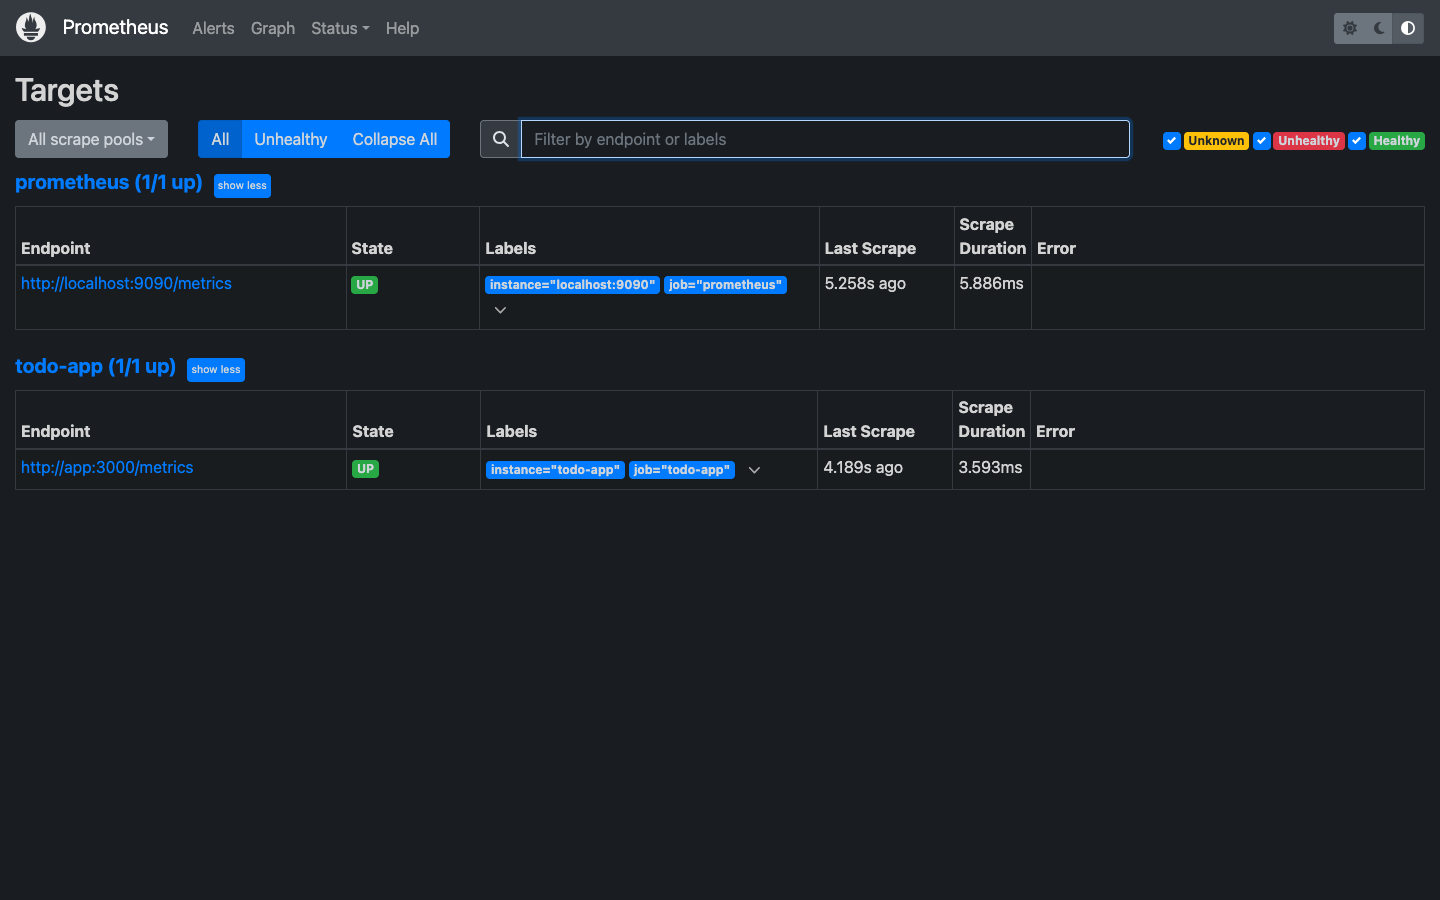
\includegraphics[width=0.95\textwidth]{prometheus_targets.png}
\caption{Prometheus targets page showing both scrape targets in UP state}
\label{fig:prom_targets}
\end{figure}

Figure \ref{fig:prom_table} shows the result of querying \texttt{http\_requests\_total} in the Prometheus expression browser after a load test. The metric is correctly labelled by \texttt{instance}, \texttt{job}, \texttt{method}, \texttt{route}, and \texttt{status\_code}, demonstrating that the custom counter captures the full dimensionality of the traffic. Observed counts include 160 health checks, 205 metrics scrapes, 92 root-route requests, 30 successful \texttt{POST /todos} creations, and 15 intentional 404 responses.

\begin{figure}[H]
\centering
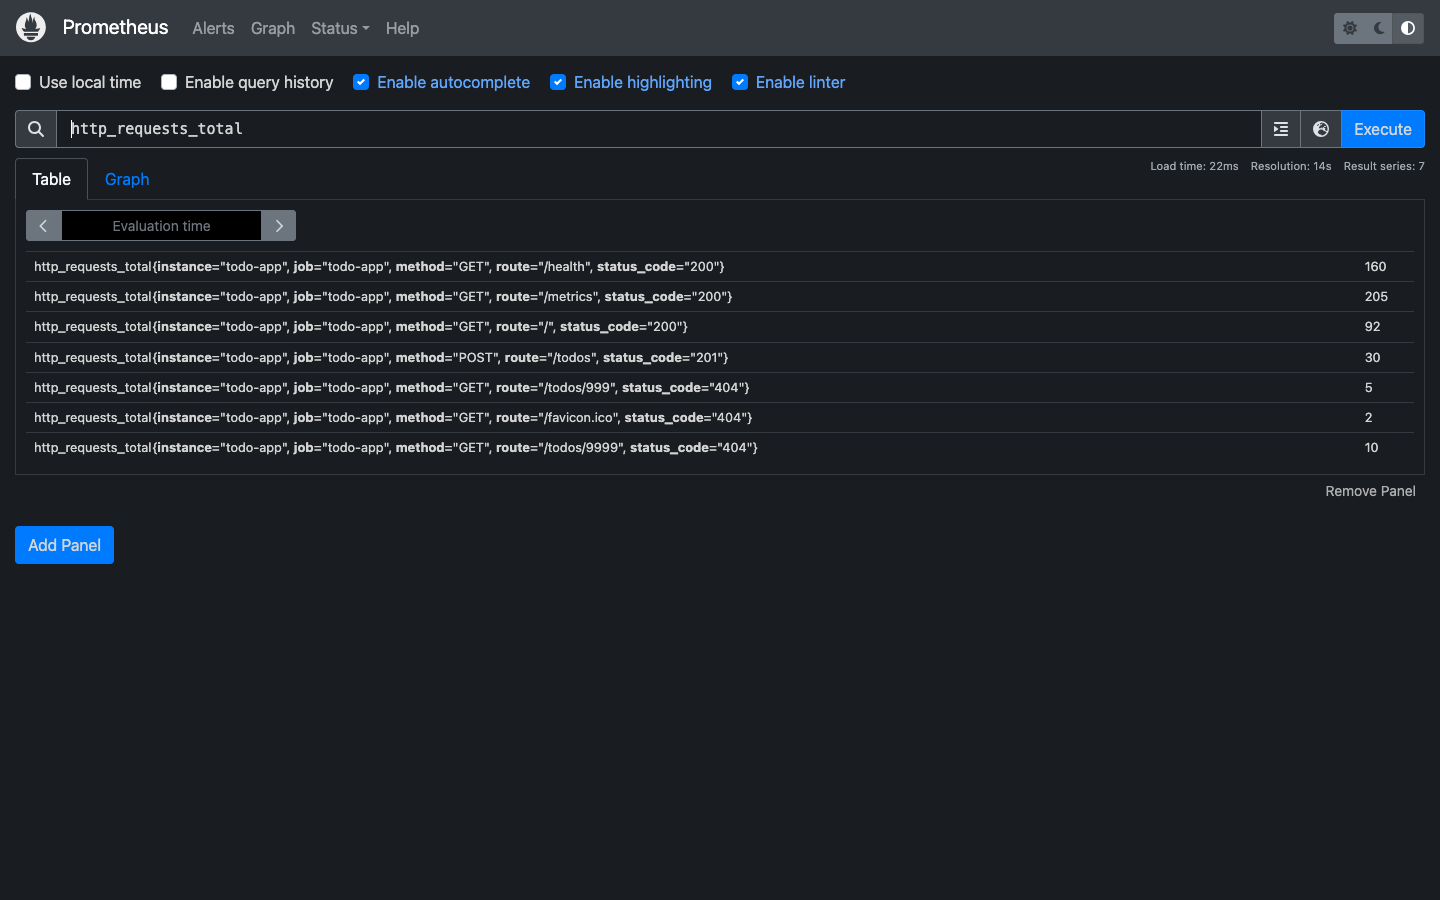
\includegraphics[width=0.95\textwidth]{prometheus_requests_table.png}
\caption{Prometheus expression browser: \texttt{http\_requests\_total} with per-route and per-status-code labels}
\label{fig:prom_table}
\end{figure}

Figure \ref{fig:prom_rate} shows the \texttt{rate(http\_requests\_total[2m])} graph over a 15-minute window. The chart clearly shows a flat baseline followed by a sharp spike during the load test burst, with the green line (\texttt{GET /}) reaching approximately 0.55 req/s and the red line (\texttt{GET /health}) reaching 0.40 req/s. The spike subsides cleanly after the burst completes.

\begin{figure}[H]
\centering
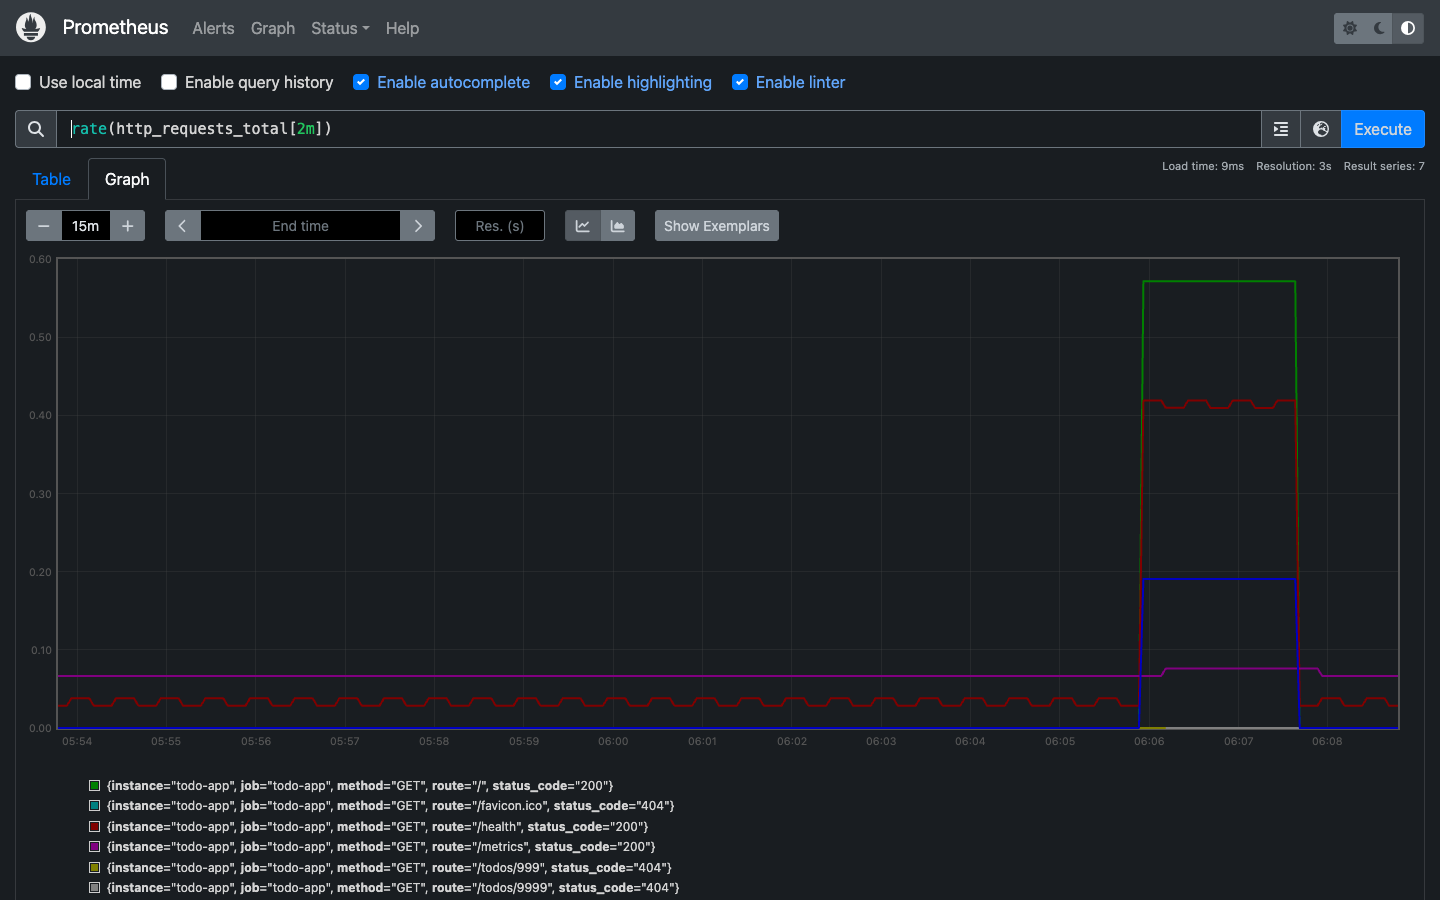
\includegraphics[width=0.95\textwidth]{prometheus_rate_graph.png}
\caption{Prometheus graph: per-route HTTP request rate (req/s) over 15 minutes}
\label{fig:prom_rate}
\end{figure}

\section{Grafana Dashboard Observations}

Figure \ref{fig:grafana} shows the auto-provisioned Grafana dashboard \textit{To-Do App Metrics} with all four panels populated with real data from the running application.

\begin{figure}[H]
\centering
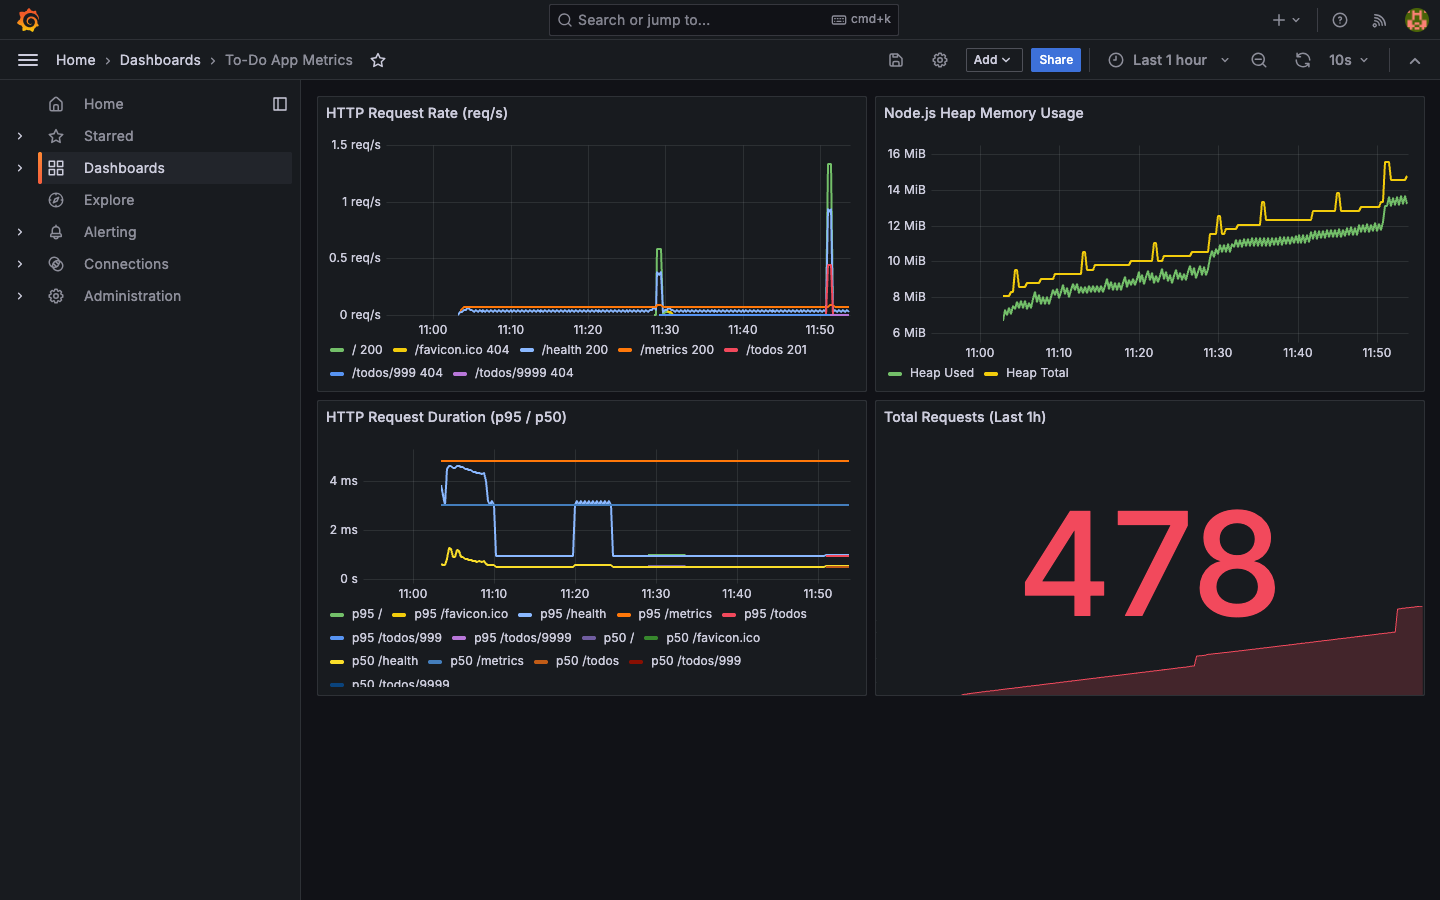
\includegraphics[width=0.95\textwidth]{grafana_dashboard.png}
\caption{Grafana dashboard showing HTTP request rate, heap memory, request duration, and total requests}
\label{fig:grafana}
\end{figure}

The four panels reveal the following observations from the actual run:

\begin{enumerate}
    \item \textbf{HTTP Request Rate (top-left)}: During the load burst, the \texttt{GET /} route peaked at approximately 1.5 req/s and \texttt{GET /health} at around 1.0 req/s. All routes are individually identifiable by their legend labels, including the 404 routes (\texttt{/todos/999}, \texttt{/todos/9999}).

    \item \textbf{Node.js Heap Memory (top-right)}: Heap Used (green) ranged between 6 MiB at idle and 14 MiB under load. Heap Total (yellow) grew from approximately 8 MiB to 16 MiB, demonstrating that Node.js dynamically expands the heap to accommodate the workload before the garbage collector reclaims unused memory.

    \item \textbf{HTTP Request Duration p95/p50 (bottom-left)}: The p95 latency for all routes remained consistently below 4 ms throughout the observation window, and the p50 (median) stayed below 1 ms. This confirms that the in-memory application introduces negligible latency under the tested load.

    \item \textbf{Total Requests (bottom-right)}: The stat panel recorded \textbf{478 total requests} in the last hour, reflecting the full traffic generated across all routes during the demonstration.
\end{enumerate}

\section{Discussion}
The project successfully demonstrates all stated objectives with real, observable evidence. Key observations:
\begin{enumerate}
    \item \textbf{Pipeline-as-code}: Storing the Jenkinsfile in the repository enables pipeline changes to go through the same review process as application code, creating a single source of truth for both application and delivery logic.
    \item \textbf{Idempotent deployment}: Running the Ansible playbook twice against the same server produces identical results, satisfying the idempotency requirement.
    \item \textbf{Observability}: The pre-provisioned Grafana dashboard provides immediate visibility without any manual configuration, demonstrating the value of monitoring-as-code. The dashboard loaded with live data within seconds of the stack starting.
    \item \textbf{Test gating}: All five Jest tests pass in under 250 ms. A deliberate endpoint break was confirmed to abort the pipeline at the test stage without touching the deployed image.
    \item \textbf{Deployment downtime}: The current stop-then-start container swap introduces a few seconds of unavailability. A true zero-downtime strategy would require a load balancer and rolling update mechanism such as Kubernetes rolling deployments.
\end{enumerate}

%% ═══════════════════════════════════════════════════════════════════════════
%%  CHAPTER 7 — CONCLUSION
%% ═══════════════════════════════════════════════════════════════════════════
\chapter{Conclusion}

\section{Summary}
This project designed and implemented a complete, production-aware CI/CD pipeline for a containerised Node.js To-Do application. The pipeline integrates GitHub, Jenkins, Docker, Docker Hub, Ansible, Prometheus, and Grafana into a cohesive automated system. Key achievements include:

\begin{enumerate}
    \item Automated build and test execution on every code push, with test failures preventing deployment.
    \item Reproducible Docker images pushed to a public registry and deployed via idempotent Ansible playbooks.
    \item Real-time monitoring with pre-provisioned Grafana dashboards showing the Four Golden Signals.
    \item All configuration stored as code in version control, enabling auditability and reproducibility.
\end{enumerate}

\section{Limitations}
\begin{enumerate}
    \item \textbf{Brief deployment downtime}: The stop-then-start container swap introduces a few seconds of unavailability.
    \item \textbf{Single-node deployment}: The Ansible inventory targets a single server; there is no horizontal scaling.
    \item \textbf{No alerting}: Prometheus alerting rules and Alertmanager integration are not implemented.
    \item \textbf{No secrets management}: Ansible vault or HashiCorp Vault could further secure sensitive variables.
    \item \textbf{No staging environment}: The pipeline deploys directly to the single target server without a separate staging gate.
\end{enumerate}

\section{Future Work}
\begin{enumerate}
    \item Migrate to \textbf{Kubernetes} (e.g., k3s or EKS) for rolling deployments, autoscaling, and self-healing.
    \item Add \textbf{Prometheus Alertmanager} rules for error-rate and latency SLO violations with PagerDuty/Slack notifications.
    \item Integrate \textbf{SonarQube} static analysis and \textbf{Trivy} container vulnerability scanning as additional pipeline stages.
    \item Implement a \textbf{staging to production promotion} workflow requiring manual approval in Jenkins.
    \item Replace the in-memory data store with a persistent \textbf{PostgreSQL} or \textbf{MongoDB} container managed via Docker Compose.
    \item Explore \textbf{GitOps} workflows using ArgoCD or Flux to replace the Ansible push-based deployment model.
\end{enumerate}

%% ═══════════════════════════════════════════════════════════════════════════
%%  REFERENCES
%% ═══════════════════════════════════════════════════════════════════════════
\bibliographystyle{plain}
\begin{thebibliography}{99}

\bibitem{jenkins_docs}
Jenkins Project.
\textit{Jenkins User Documentation}.
Available: \url{https://www.jenkins.io/doc/}.
Accessed: May 2026.

\bibitem{docker_docs}
Docker Inc.
\textit{Docker Documentation}.
Available: \url{https://docs.docker.com/}.
Accessed: May 2026.

\bibitem{prometheus_docs}
Prometheus Authors.
\textit{Prometheus Documentation}.
Available: \url{https://prometheus.io/docs/}.
Accessed: May 2026.

\bibitem{grafana_docs}
Grafana Labs.
\textit{Grafana Documentation}.
Available: \url{https://grafana.com/docs/grafana/latest/}.
Accessed: May 2026.

\bibitem{ansible_docs}
Red Hat Inc.
\textit{Ansible Documentation}.
Available: \url{https://docs.ansible.com/}.
Accessed: May 2026.

\bibitem{github_actions_docs}
GitHub Inc.
\textit{GitHub Actions Documentation}.
Available: \url{https://docs.github.com/en/actions}.
Accessed: May 2026.

\bibitem{gitlab_ci_docs}
GitLab Inc.
\textit{GitLab CI/CD Documentation}.
Available: \url{https://docs.gitlab.com/ee/ci/}.
Accessed: May 2026.

\bibitem{kim2016devops}
G. Kim, J. Humble, P. Debois, and J. Willis.
\textit{The DevOps Handbook: How to Create World-Class Agility, Reliability, and Security in Technology Organisations}.
IT Revolution Press, Portland, OR, 2016.

\bibitem{beyer2016sre}
B. Beyer, C. Jones, J. Petoff, and N. R. Murphy, Eds.
\textit{Site Reliability Engineering: How Google Runs Production Systems}.
O'Reilly Media, Sebastopol, CA, 2016.

\bibitem{humble2010continuous}
J. Humble and D. Farley.
\textit{Continuous Delivery: Reliable Software Releases through Build, Test, and Deployment Automation}.
Addison-Wesley, Upper Saddle River, NJ, 2010.

\end{thebibliography}

\end{document}
